% Uncomment this to make slides with overlays:
%\documentclass[slides]{beamer}

% Uncomment these (but comment the above \documentclass line) to make handouts:
\documentclass[handout]{beamer}

% Uncomment these to have more than one slide per page
\usepackage{pgfpages}
\pgfpagesuselayout{2 on 1}[border shrink=5mm]
\pgfpageslogicalpageoptions{1}{border code=\pgfusepath{stroke}}
\pgfpageslogicalpageoptions{2}{border code=\pgfusepath{stroke}}

\usepackage[]{graphicx, color, hyperref}

\mode<presentation>
{
	%\usetheme[secheader]{Boadilla}
	%\usecolortheme[rgb={.835, .102,.169}]{structure}  
	\usetheme[width= 0cm]{Goettingen}
	%\setbeamercovered{transparent}
}
\setbeamertemplate{navigation symbols}{}
\setbeamertemplate{footline}[frame number]

\definecolor{blue2}{rgb}{0.278,0.278,0.729} 
\newcommand{\blue}[1]{\textcolor{blue2}{#1}}
\newcommand{\white}[1]{\textcolor{white}{#1}}
\newcommand{\red}[1]{\textcolor{red}{#1}}
\newcommand{\xbar}{\overline{x}}
\newcommand{\ybar}{\overline{y}}
\newcommand{\phat}{\widehat{p}}
\newcommand{\prob}{\mbox{Pr}}
\newcommand{\E}{\mathbb{E}}
\newcommand{\Var}{\mbox{Var}}
\newcommand{\cp}{\oplus}
\newcommand{\cm}{\circleddash}

\title{Lecture 11: Binomial and Poisson Random Variables}
\author{Chapter 3.3-3.5}
\date{}


\begin{document}
%------------------------------------------------------------------------------
\begin{frame}
\titlepage
\end{frame}
%------------------------------------------------------------------------------


%------------------------------------------------------------------------------
\begin{frame}[fragile]
\frametitle{Goals for Today}

Define
\begin{itemize}
\item Binomial random variables
\item Poisson random variables
\end{itemize}


\end{frame}
%------------------------------------------------------------------------------


%------------------------------------------------------------------------------
\begin{frame}
\frametitle{Binomial Distribution}

So say now, instead of $P(\mbox{1st W in 5th game}) = P(\mbox{\blue{LLLLW}})$, we want the probability that they win \blue{exactly one} out of the five games.  Five ways:

\pause\begin{center}
\begin{tabular}{c|ll}
Pattern & Probability & Equals\\
\hline
\blue{WLLLL} & $p \times (1-p)^4$ & $=p\times(1-p)^4$\\
\blue{LWLLL} & $(1-p) \times p \times (1-p)^3$ & $=p\times(1-p)^4$\\
\blue{LLWLL} & $(1-p)^2 \times p \times (1-p)^2$& $=p\times(1-p)^4$\\
\blue{LLLWL} & $(1-p)^3 \times p \times (1-p)$& $=p\times(1-p)^4$\\
\blue{LLLLW} & $(1-p)^4 \times p$& $=p\times(1-p)^4$\\
\end{tabular} 
\end{center}

\pause Each pattern (book calls it scenario) has the same probability regardless of order by independence, and there are 5 ways to \blue{choose} the pattern.

\vspace{0.25cm}

\pause So $P(\mbox{win exactly one out of five})$ is  $5 \times p\times(1-p)^4 = 5 \times 0.4^4 \times 0.6 = 0.0768$

\end{frame}
%------------------------------------------------------------------------------



%------------------------------------------------------------------------------
\begin{frame}
\frametitle{Step Back... Example of $n$ choose $k$}
Say I give you $n=5$ balls labeled 1 thru 5.  How many different ways can you choose $k=3$ of them?

\begin{center}
\pause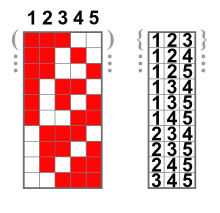
\includegraphics[height=4cm]{figure/choose.png}
\end{center}

As we see, 10 ways.  

\end{frame}
%------------------------------------------------------------------------------



%------------------------------------------------------------------------------
\begin{frame}
\frametitle{Step Back... $n$ choose $k$ in General}
Say I give you $n$ balls labeled 1 thru n.  How many different ways can you choose $k$ of them?

\[
{n \choose k} = \frac{n!}{k!(n-k)!}
\]

This is read \blue{n choose k}.  

\pause \vspace{0.5cm}

In example: $n=5$ and $k=3$
\[
{5 \choose 3} = \frac{5!}{3!(5-3)!} = \frac{5 \times 4 \times 3 \times 2 \times 1}{(3 \times 2 \times 1)(2 \times 1)} = \frac{120}{12} = 10
\]

Note that $0!=1$

\end{frame}
%------------------------------------------------------------------------------


%------------------------------------------------------------------------------
\begin{frame}
\frametitle{Binomial Distribution}
Suppose the probability of a single trial being a success is $p$.  Then the probability of observing exactly $k$ successes in $n$ independent trials is given by:

\pause\begin{eqnarray*}
P(\mbox{exactly $k$ successes}) &=& {n \choose k} p^k (1-p)^{n-k}\\
&=& \frac{n!}{k!(n-k)!}p^k (1-p)^{n-k}
\end{eqnarray*}

\pause The mean, variance, and SD are:
\[
\mu = np \hspace{1cm} \sigma^2 = np(1-p) \hspace{1cm} \sigma = \sqrt{np(1-p)}
\]

\end{frame}
%------------------------------------------------------------------------------


%------------------------------------------------------------------------------
\begin{frame}
\frametitle{Conditions for Binomial Distribution}

\begin{enumerate}
\pause\item The trials are independent.
\pause\item The number of trials $n$ is fixed
\pause\item Each trial outcome can be classified as a failure or a success
\pause\item The probability of a success $p$ is the same for each trial
\end{enumerate}

\end{frame}
%------------------------------------------------------------------------------


%------------------------------------------------------------------------------
\begin{frame}
\frametitle{Back to Soccer Example}
The Portland Timbers have equal probability p = 0.6 of winning any particular soccer game. We want the probability that they win \blue{exactly one} out of the five games.  Five ways:

\pause\begin{center}
\begin{tabular}{c|ll}
Pattern & Probability & Equals\\
\hline
\blue{WLLLL} & $p \times (1-p)^4$ & $=p\times(1-p)^4$\\
\blue{LWLLL} & $(1-p) \times p \times (1-p)^3$ & $=p\times(1-p)^4$\\
\blue{LLWLL} & $(1-p)^2 \times p \times (1-p)^2$& $=p\times(1-p)^4$\\
\blue{LLLWL} & $(1-p)^3 \times p \times (1-p)$& $=p\times(1-p)^4$\\
\blue{LLLLW} & $(1-p)^4 \times p$& $=p\times(1-p)^4$\\
\end{tabular} 
\end{center}

\pause Letting a win be a ``success'':
\begin{eqnarray*}
P(\mbox{$k=1$ win}) &=& {n \choose k} p^k (1-p)^{n-k} = \frac{5!}{1!\times4!} 0.6 \times 0.4^4\\
&=& 5 \times  0.6 \times 0.4^4 = 0.0768
\end{eqnarray*}

\end{frame}
%------------------------------------------------------------------------------


%------------------------------------------------------------------------------
\begin{frame}
\frametitle{Back to Soccer Example}
What about the probability that they win all their games!  i.e. $k=5$:
\pause \begin{eqnarray*}
P(\mbox{$k=5$ wins}) &=& {n \choose k} p^k (1-p)^{n-k} = {5 \choose 5} 0.6^5 (1-0.6)^{0}\\
&=& \frac{5!}{5!\times 0!} 0.6^5 \times 1 = 0.08
\end{eqnarray*}

\vspace{0.75cm}

\pause What about the probability that they at win at least one game?
\pause \begin{eqnarray*}
P(\mbox{at least $k=1$ wins}) &=& P(\mbox{$k=1$ win}) + \ldots + P(\mbox{$k=5$ wins}) \\
&=& 1 - P(\mbox{k=0 wins})\\
&=& 1 -  \frac{5!}{0!\times 5!} 0.6^0 \times 0.4^5 = 1 - 0.01024\\
&=& 0.98976
\end{eqnarray*}


\end{frame}
%------------------------------------------------------------------------------


%pdf("./5.1 Binomial+Poisson/bin.pdf", width=7, height=5)
%x <- c(0:5)
%y <- dbinom(x, size=5, prob=0.6)
%plot(x,y, xlab="k: number of successes", ylab="P(k successes)", ylim=c(0, max(y)))
%points(x,y, pch=19, cex=1.5)
%dev.off()
%------------------------------------------------------------------------------
\begin{frame}
\frametitle{Back to Soccer Example}

\begin{center}
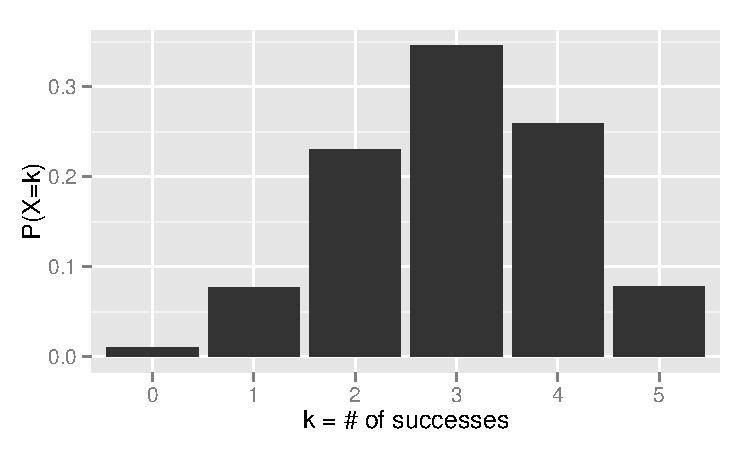
\includegraphics[width=8cm]{figure/bin.pdf}
\end{center}

\end{frame}
%------------------------------------------------------------------------------


%------------------------------------------------------------------------------
\begin{frame}
\frametitle{Poisson Distribution}

Say you want to count the number of rare events in a large population over a unit of time.  Examples:
\begin{itemize}
\pause \item the number of car accidents at a particular intersection on a given week
\pause \item the number of ambulance calls on any given day in Portland
\pause \item the number of soldiers in the Prussian army killed accidentally by horse kick from 1875 to 1894
\end{itemize}

\vskip 0.25cm

\pause The \blue{Poisson distribution} helps us describe the number of such events that will occur in a short unit of time for a fixed population if the individuals within the population are
independent.

\end{frame}
%------------------------------------------------------------------------------


%------------------------------------------------------------------------------
\begin{frame}
\frametitle{Poisson Distribution}
Suppose we are watching for rare events and the number of observed events follows a Poisson distribution with rate $\lambda$
\[
    P(\mbox{observe k rare events}) = \frac{\lambda^k e^{-\lambda}}{k!}
\]
\pause where k may take a value 0, 1, 2, \ldots where $e \approx 2.718$.

\vspace{0.5cm}

\pause The mean and SD are $\lambda$ and $\sqrt{\lambda}$.

\end{frame}
%------------------------------------------------------------------------------


%------------------------------------------------------------------------------
\begin{frame}
\frametitle{Conditions for Poisson Distribution}
A random variable \blue{may} be Poisson distributed if

\begin{enumerate}
\pause\item The event in question is rare
\pause\item The population is large
\pause\item The events occur independently of each other
\end{enumerate}

\end{frame}
%------------------------------------------------------------------------------


%------------------------------------------------------------------------------
\begin{frame}
\frametitle{Exercise 3.47 on Page 158}
A coffee shop serves an average of 75 customers per hour during the morning rush.  What is the probability that the coffee shop serves 70 customers in one hour during this time of the day?

\vspace{0.5cm}

\pause In this case, $\lambda=75$ is the rate
\[
P(k=70) = \frac{75^{70} e^{-75}}{70!} = 0.040
\]

\pause\vspace{0.25cm}

Type {\tt dpois(x=70, lambda=75)} in {\tt R}

\end{frame}
%------------------------------------------------------------------------------


%------------------------------------------------------------------------------
\begin{frame}[fragile]
\frametitle{Next Time}

Chapter 4:  Foundations for Inference
\begin{itemize}
\item Variability in estimates $\overline{x}$, $\widehat{p}$, etc.
\item In fact, we can associate a \blue{distribution} to these estimates
\end{itemize}


\end{frame}
%------------------------------------------------------------------------------



\end{document}


